% 여기서 앞서 정리한 부분의 결과를 확인하는 section 으로 사용한다. -> 다음 
\vspace{-6mm}
\subsection{}
\vspace{-2mm}
\subsubsection{Simulation Results : 채널 효율}
\vspace{-2mm}
    Aloha 와 Slotted aloha를 비교해 주기 위해서 Throughput 을 매개로 G-load 에 따른 비교이기 때문에 Throughput 과 같은 값이라고 할 수 있는 채널효율의 값을 확인해 분석을 하였다.
    Results 에 생성된 sca, 스칼라 파일로부터 aloha server에서 채널 효율값을 확인해 주었다. 
    각각의 scalar 파일을 csv로 변환하여 직접 graph를 그려 분석하려 했으나 \mintinline{c}{scavedata.cc}가 정상적으로 실행되지 않아 sca 에서 직접 확인한 값을 캡처했다.
\vspace{-2mm} 
        \begin{figure}[h!]
        \centering
        \subfloat[Expeitiment 1-1 pure aloha’s Channel Utilizaiton : 0.116946]{
            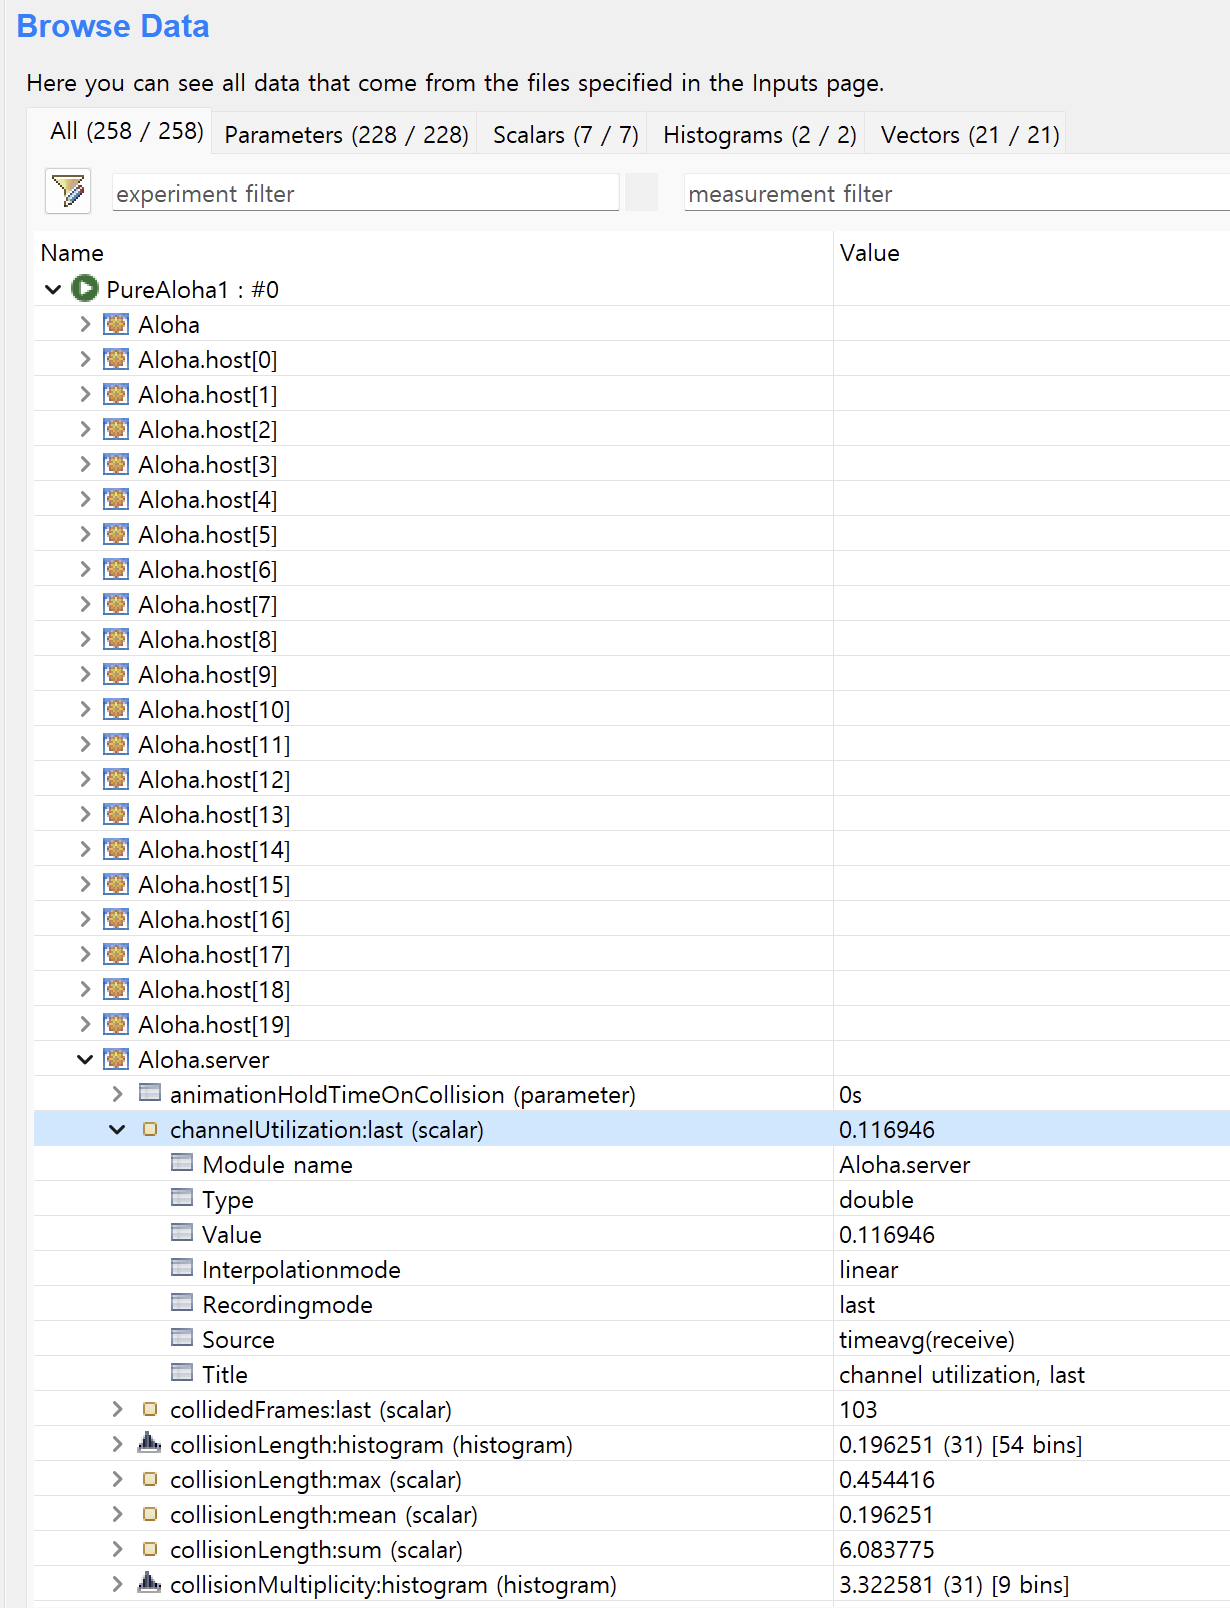
\includegraphics[width=0.43\textwidth]{image/week12/1-2-1.png}
        }\hspace{8mm}
        \subfloat[Expeitiment 1-2 pure aloha’s Channel Utilizaiton : 0.172417]{
            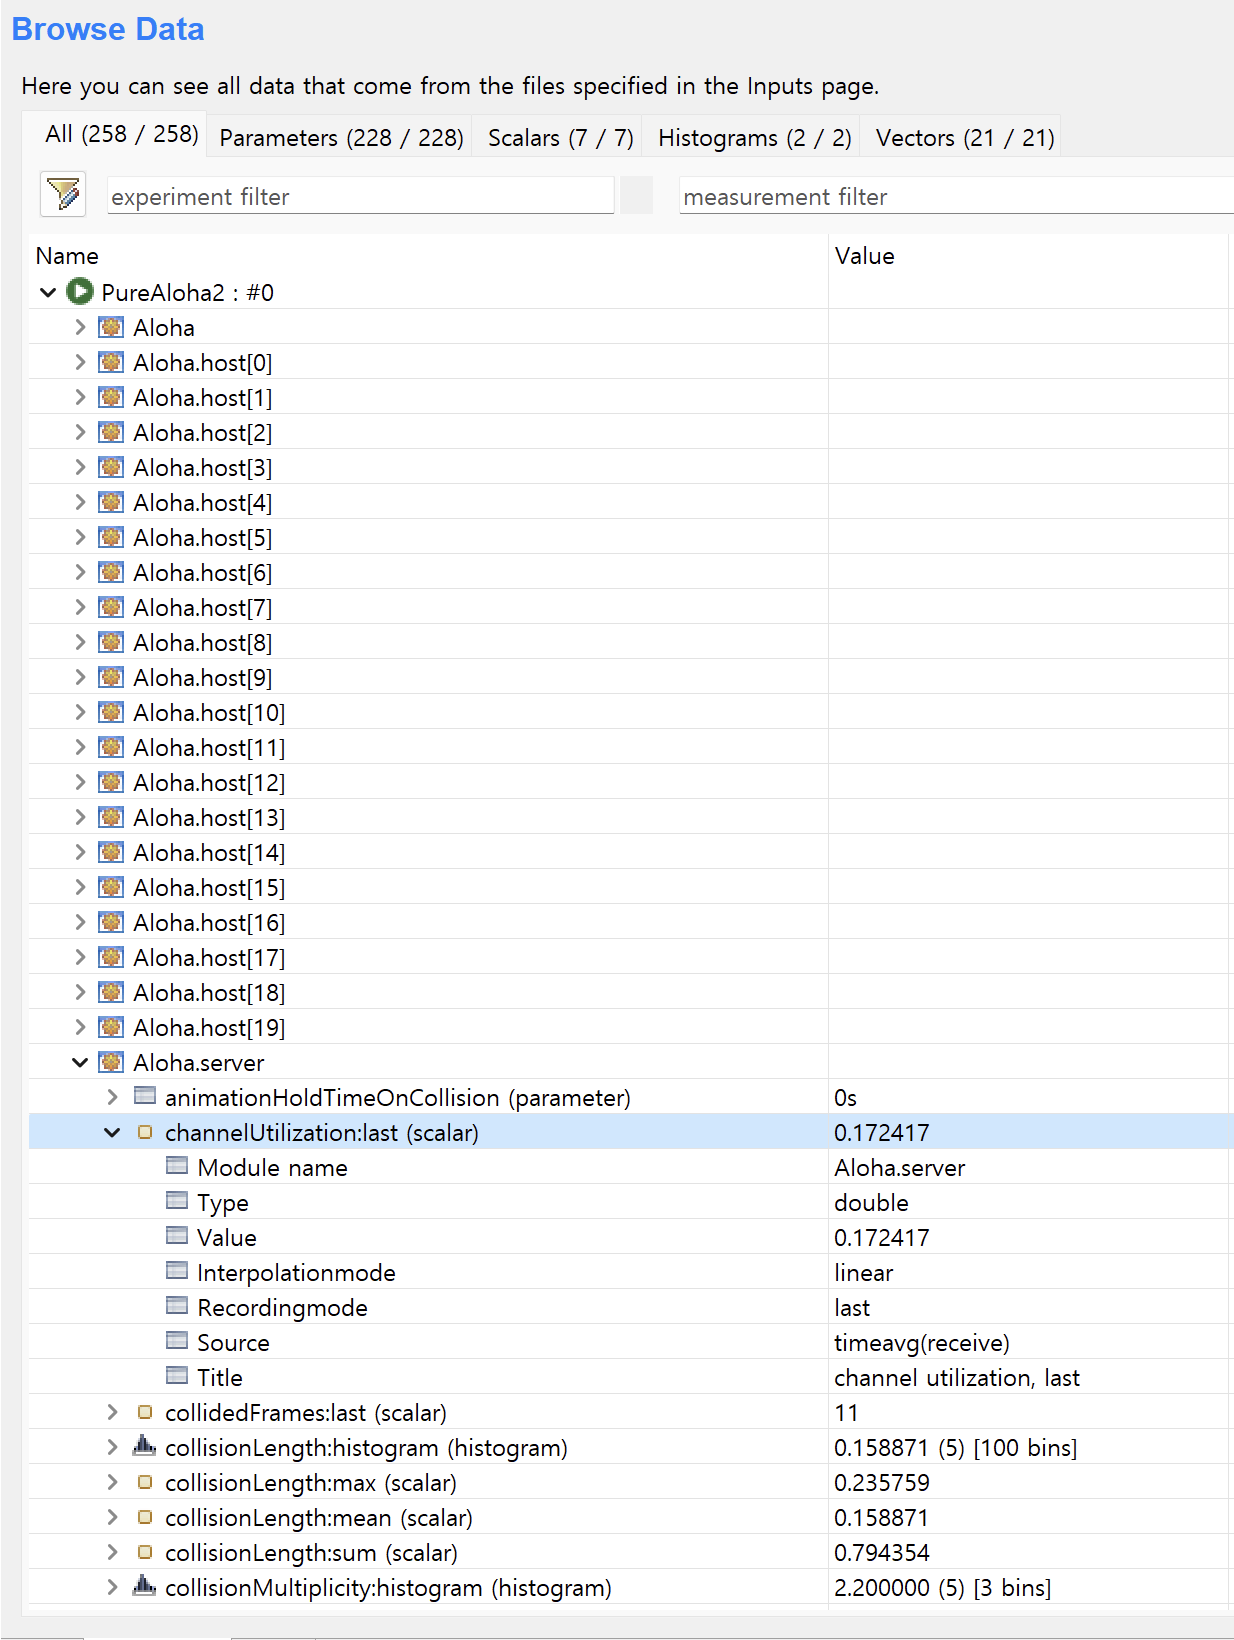
\includegraphics[width=0.43\textwidth]{image/week12/1-2-2.png}
        }\hspace{3mm}
        \subfloat[Expeitiment 1-3 slotted aloha’s Channel Utilizaiton : 0.108012]{
            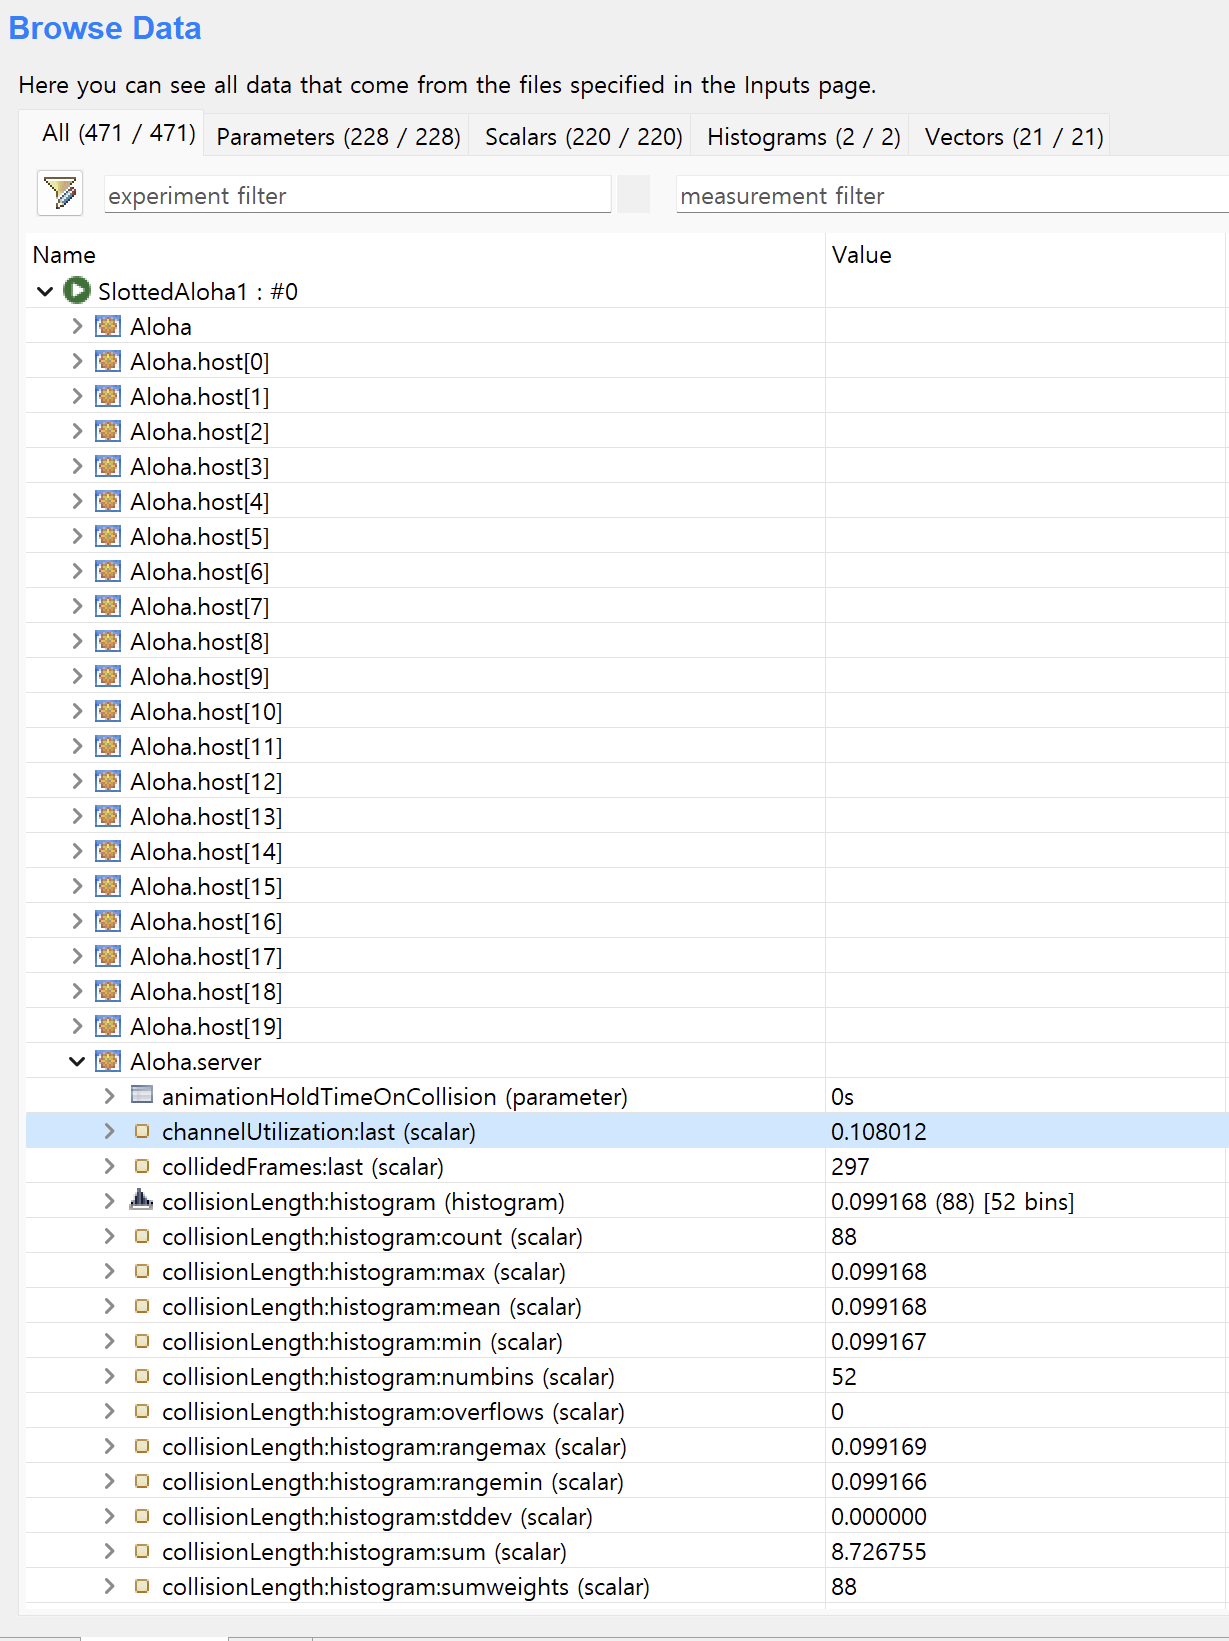
\includegraphics[width=0.43\textwidth]{image/week12/1-2-3.png}
        }\hspace{8mm}
        \subfloat[Expeitiment 1-4 slotted aloha’s Channel Utilizaiton : 0.30498]{
            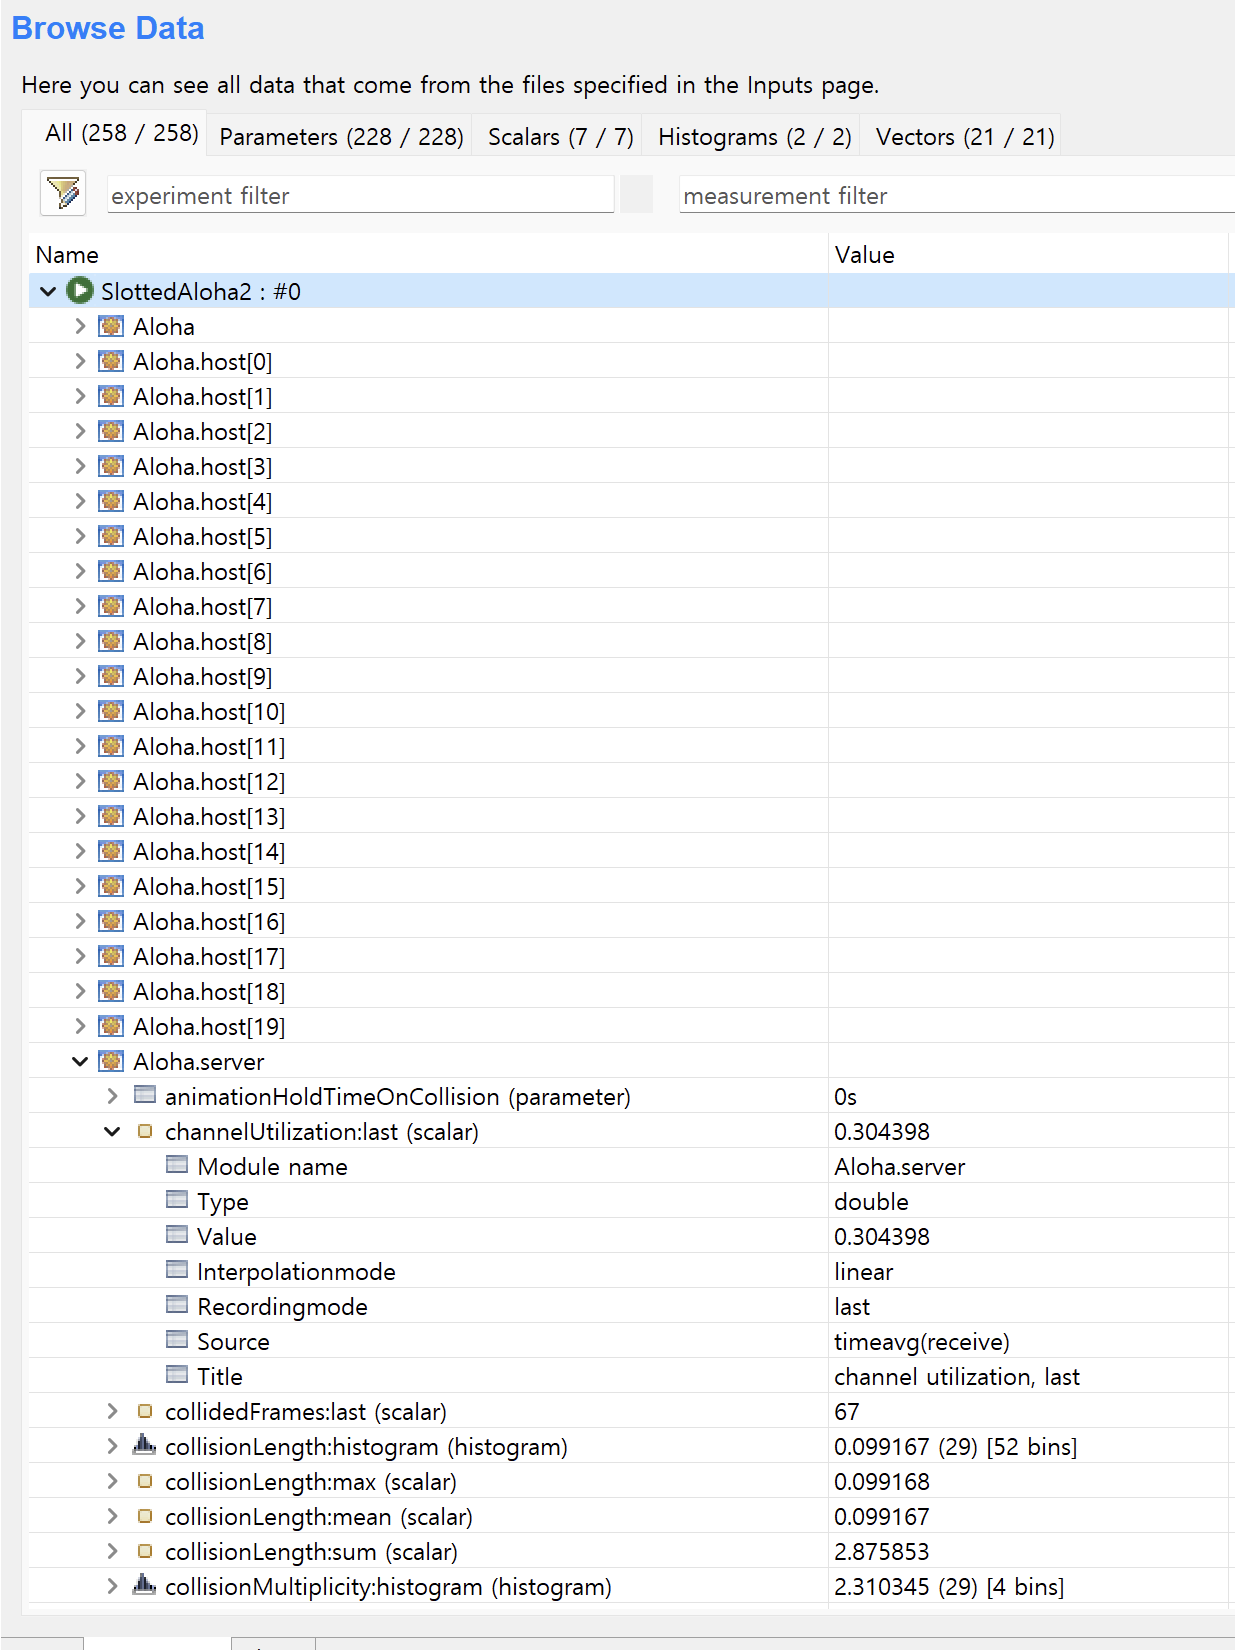
\includegraphics[width=0.43\textwidth]{image/week12/1-2-4.png}
        }
        \vspace{-2mm}
        \caption{Experiment 1-1 Simulation Results Screenshot: packetReceived}
        \end{figure}
    \vspace{-3mm}
\subsubsection{Discussion}
%%------------------------------------------------------------------------------------------
%                                   section intro 2 column
%%------------------------------------------------------------------------------------------
\begin{multicols}{2}
    \begin{minipage}{\columnwidth}
    \vspace{2mm}
    \centering%
    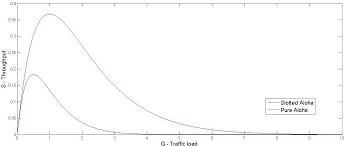
\includegraphics[width=.99\textwidth]{image/week12/1-3.png}
    \vspace{-2mm}
    \captionof{figure}{\small Aloha Throughput Graph depend on G-load}    \vspace{-4mm}
    \end{minipage}
    
    \columnbreak
    
    aloha와 slotted aloha의 차이를 확인하고자 측정한 4가지 조건의 throughput인 채널효율로 부터 pure aloha와 slotted aloha의 각각의 vulnerable time이 2배 차이로 부터 G-load에 상응하는 포아송분포로 표현한 throughput 의 graph와 측정값이 유사하게 나옴으로서 확인했다.
    $$
    S(\text{throughput})= P_{\text{success}} \times G =
    \begin{cases}
    \frac{(2G)^k}{k!}e^{-2G}, & \mbox{pure aloha case}\\
    \frac{(G)^k}{k!}e^{-G}, & \mbox{slotted aloha case}
    \end{cases}
    $$
    \vspace{-4mm}
\end{multicols}
\vspace{-3mm}


